\documentclass[11pt,a4paper]{article}
\usepackage[margin=0.75in]{geometry}
\usepackage{graphicx}
\usepackage{float}
\usepackage{caption}
\usepackage{subcaption}
\usepackage{amsmath}
\usepackage{booktabs}
\usepackage[hidelinks]{hyperref}
\begin{document}

In our last dicussion, The Disease detetion model I tranied was achieved \textbf{100\% test accuracy}, which was raised as concern. Following your feedbacks, I did detailed investigation on the datasetand the training configurations. In the training process, I identified two issues:
\begin{enumerate}
    \item \textbf{Excessive Training}: The large number of training epochs (130 epochs) was causing the model to overfit on the relatively small laboratory-scale leaf image dataset.
    
    \item \textbf{Insufficient Regularization}: The dropout rate was initially set to 0.2, which proved inadequate for the classifier head. Given the significant number of parameters in the classification layer, the network was able to memorize training patterns too easily.
\end{enumerate}

\section*{Solution}

\begin{itemize}
    \item \textbf{Increased dropout rate from 0.2 to 0.5} (to enhance regularization)
    \item \textbf{Reduced the total number of training epochs from 130 to 40} (to prevent overfitting)
\end{itemize}

By modifying these configurations, the model achieved \textbf{$99.8\%\pm0.05$} test accuracy over 5 runs

\section*{Model training curves comparison}

Figure~\ref{fig:comparison} shows the training curves before and after configuration updates. In \textbf{figure a:} the learning curves flattened after approximately at epoch 35, beyond that there is no significant improvement up-to epoch 130. In \textbf{figure b:} The updated training configuration exhibits healthier training curves.
\begin{figure}[H]
    \centering
    \begin{subfigure}[b]{0.7\textwidth}
        \centering
        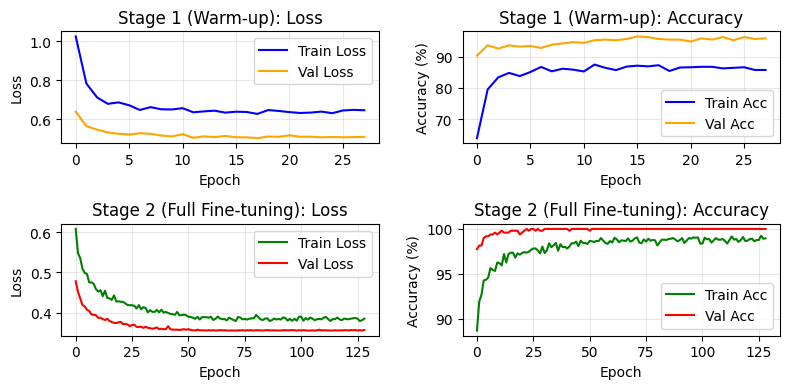
\includegraphics[width=\textwidth]{results/mobilenet_128learning.png}
        \caption{traning curves with 130 epochs and dropout rate 0.2 (100\% test accuracy);}
        \label{fig:original}
    \end{subfigure}
    \vfill
    \begin{subfigure}[b]{0.6\textwidth}
        \centering
        
\includegraphics[width=\textwidth]{results/seed789/mobilenet_training_curves.png}
        \caption{traning curves with 40 epochs and dropout rate 0.5 (99.75\% test accuracy - better generalization)}
        \label{fig:improved} 
    \end{subfigure}
    \caption{Comparison of model training/learning curves showing impact of limited training epochs and higher dropout rate.}
    \label{fig:comparison}
\end{figure}

\section*{Model evaluation on the test set}

The final model (MobileNetV2-128x128) was evaluated on 814 test images (totally unseen during training), on 4 disease classes:

\subsection*{Overall Performance}
\textbf{Test Accuracy:} 99.75\% | \textbf{F1-score:} 0.9980 | \textbf{Precision:} 0.9982 | \textbf{Recall:} 0.9979
\begin{table}[H]
\begin{tabular}{@{}lcccc@{}}
\toprule
\textbf{Class} & \textbf{Precision} & \textbf{Recall} & \textbf{F1-Score} & \textbf{Support} \\ 
\midrule
Black rot    & 1.0000 & 0.9915 & 0.9957 & 236 \\
Esca         & 0.9928 & 1.0000 & 0.9964 & 277 \\
Healthy      & 1.0000 & 1.0000 & 1.0000 & 85  \\
Leaf blight  & 1.0000 & 1.0000 & 1.0000 & 216 \\
\midrule
\textbf{Overall} & \textbf{0.9976} & \textbf{0.9975} & \textbf{0.9975} & \textbf{814} \\
\bottomrule
\end{tabular}
\captionsetup{justification=raggedright,singlelinecheck=false}
\caption{Detailed classification metrics for each disease classes}
\label{tab:results}
\end{table}


Therefore, these configuration adjustments addressed the issue identified during the presentation. The model
now demonstrates more reliable generalization capability while maintaining good performance on grape leaf disease detection task. The slight reduction from 100\% to $99.8\%\pm0.05$ accuracy reflects safer learning and increases the confidence of the model’s ability for detecting leaf disease classes in the vineyard environment. 

\end{document}
